\documentclass[a4paper]{article}

\usepackage[spanish, es-tabla, es-nodecimaldot]{babel}
\usepackage[T1]{fontenc}
\usepackage[utf8]{inputenc}
\usepackage{lmodern}
\usepackage{amsmath, amssymb}
\usepackage{stackengine}
\usepackage{graphicx}
\usepackage[hmargin=1.8cm, vmargin=2cm]{geometry}
\usepackage[separate-uncertainty=true, per-mode=symbol]{siunitx}
\usepackage[small]{titlesec}
\usepackage[bottom]{footmisc}
\usepackage{float}
\usepackage{enumitem}
\usepackage{tikz}
\usepackage[font=small, labelfont=bf, labelsep=period]{caption}
\usepackage{subcaption}
\usepackage[colorlinks=true]{hyperref}

\newcommand{\letrita}[1]{\textsf{\textbf{\footnotesize{(#1)}}}} 

\title{\large{\textbf{Caracterización del generador de número aleatorios del Kilobot o \emph{Moneda}}}}
\author{%
	\normalsize{Tomás Ayala y Romina D'Alessandro}
}
\date{}

\begin{document}
	
\maketitle

Corrimos \href{https://github.com/rldromina/Kilobots/blob/tom/Moneda/moneda.c}{\texttt{moneda.c}}, usando siempre la función \texttt{rand\_hard()}.
Dejamos fijo el tiempo mínimo de prendido/apagado del LED del Kilobot a \texttt{TIME = 1000} (milisegundos).
Registramos varias filmaciones de 15 minutos del Kilobot ``tirando la moneda'' y una de 1 hora.

De cada medición obtenemos un \texttt{.csv} que en sus columnas tiene (i) la intensidad (en un entorno) del LED, con valores entre 0 y 255, y (ii) el instante del tiempo correspondiente.
Graficamos la evolución temporal $I(t)$, su autocorrelación (ver la función \texttt{autocorrelación} de \href{https://github.com/rldromina/Kilobots/blob/tom/Moneda/aux.py}{\texttt{aux.py}}) y la frecuencia con las que ocurren las consecutividades\footnote{¿Existe esta palabra?} de longitud $n$.
Por ejemplo, si la moneda en una tirada arrojó HTHTTTHHTHHHHHH, la consecutividad de longitud $n=1$ se presentó $4$ veces (H,T,H,T); la de $n=2$, $1$ vez (HH); la de $n=3$, 1 vez (TTT); la de $n=4$ y $n=5$, ninguna y $n=6$, 1 vez (HHHHHH).
Notar que consecutividades de cara o ceca contribuyen por igual.

\begin{figure}[!h]
	\centering
	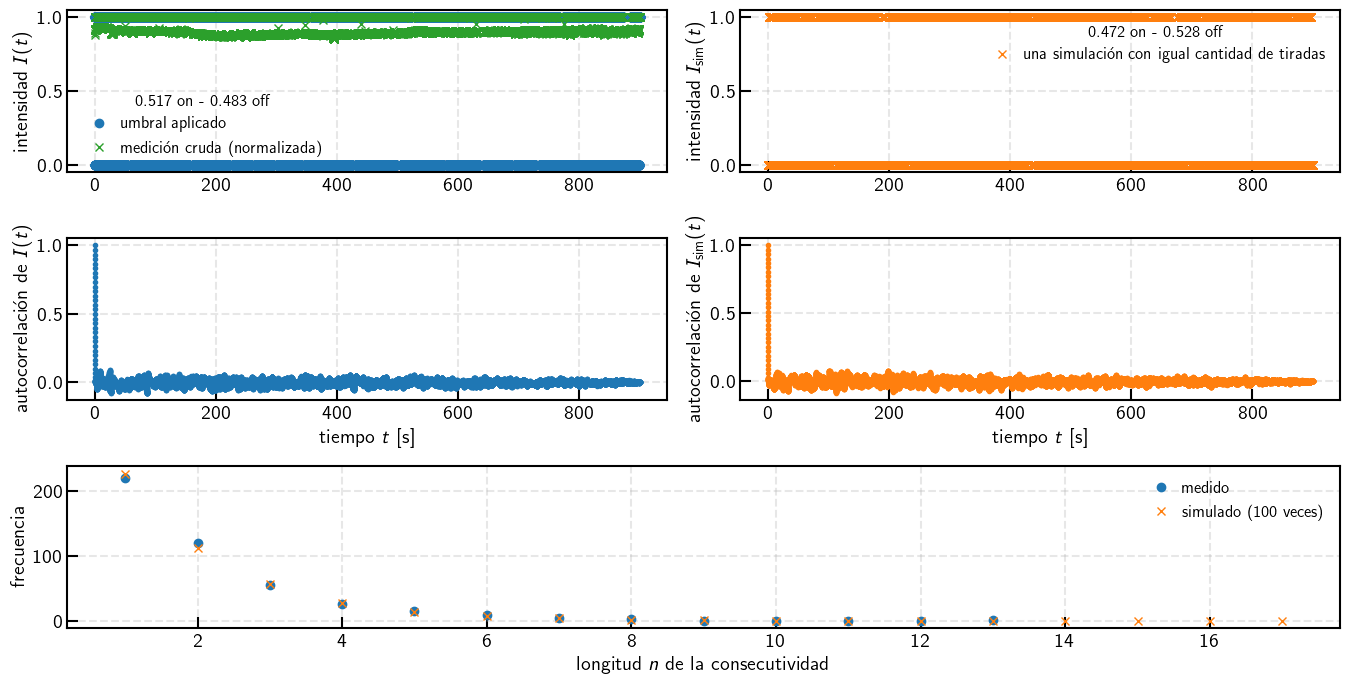
\includegraphics[width=\linewidth]{Resultados/15min_b.png}
	\caption{15 minutos, medición b.}
	\label{fig:buena_moneda}
\end{figure}

La medición cruda fue tomada, parece, con mucha luz ambiental.
Por eso cuando el LED estaba apagado, el valor de la intensidad está más cerca de saturar\footnote{Los valores presentados en verde están normalizados, o sea, divididos por 255.} (255) que de cero.
Aun así se logra distinguir los dos estados del Kilobot.
Para el análisis le pasamos un \href{https://github.com/rldromina/Kilobots/blob/tom/Moneda/aux.py}{umbral} que asigna sólo dos valores: 1 (prendido) y 0 (apagado).

En naranja se presenta el resultado de una simulación de la moneda tirada $900$ veces ya que $\SI{15}{\minute} = \SI{900}{\second}$ y era \texttt{TIME = 1000}.

Las autocorrelaciones, en ambos casos medido y simulado, caen a cero en $\SI{1}{\second}$ o, equivalentemente, luego de $30$ puntitos\footnote{Grabamos a $30$ fps y los frames los capturamos con una tasa $t = 1$, o sea, guardábamos $1$ de cada $t$ frames, quedándonos en este caso con todos los frames.}.

En Labo 7 notábamos que ocurrían consecutividades en las tiradas de longitud $n=12$ por ejemplo.
Esto nos volvía locos, por eso es parte de la caracterización medir la frecuencia con las que estas consecutividades aparecen.
También lo fue el cálculo de la autocorrelación: pensábamos que con altas consecutividades presentes, el tiempo de correlación iba a ser mayor al de una moneda ``ideal'' (i.e. simulada en python), pero no.

Nos focalizamos entonces en el conteo de consecutividades.
Para esta medición, comparamos esta frecuencia de aparición de consecutividades con las de una moneda simulada.
Presentamos, en naranja, la media de $100$ realizaciones, cada una con la misma cantidad de tiradas\footnote{Si la cantidad de tiradas es muuuy grande es posible, aunque poco probable, que aparezca una consecutividad de, por ejemplo, longitud $n=20$, lo cual es casi imposible si la cantidad de tiradas es $20$ e imposible si es menor. Por ejemplo, ocurrió por lo menos una vez una consecutividad de longitud $17$ en un alguna de las $100$ simulaciones.}.
Me sorprendió mucho que las frecuencias medidas y simuladas concuerden tan bien. 

Resumiendo, lo medido (y de lo que sospechábamos) y lo simulado presentan el mismo comportamiento:
\begin{itemize}
	\item 51.7\% on - 48.3\% off vs. 47.2\% on - 52.8\% off
	\item mismo tiempo de correlación $= \SI{1}{\second}$
	\item misma distribución de consecutividades (!)
\end{itemize}

Para las otras mediciones, los resultados fueron:

\begin{figure}[!h]
	\centering
	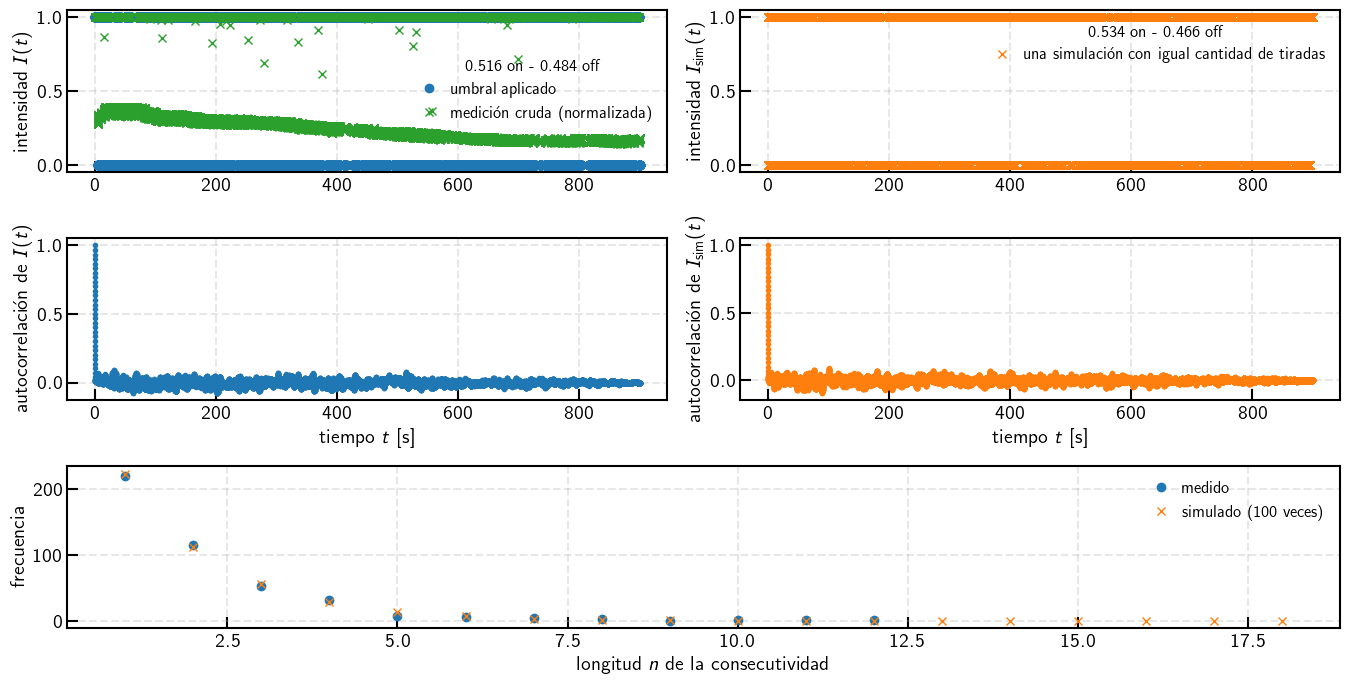
\includegraphics[width=\linewidth]{Resultados/15min_c.png}
	\caption{15 minutos, medición c.}
\end{figure}

\begin{figure}[!h]
	\centering
	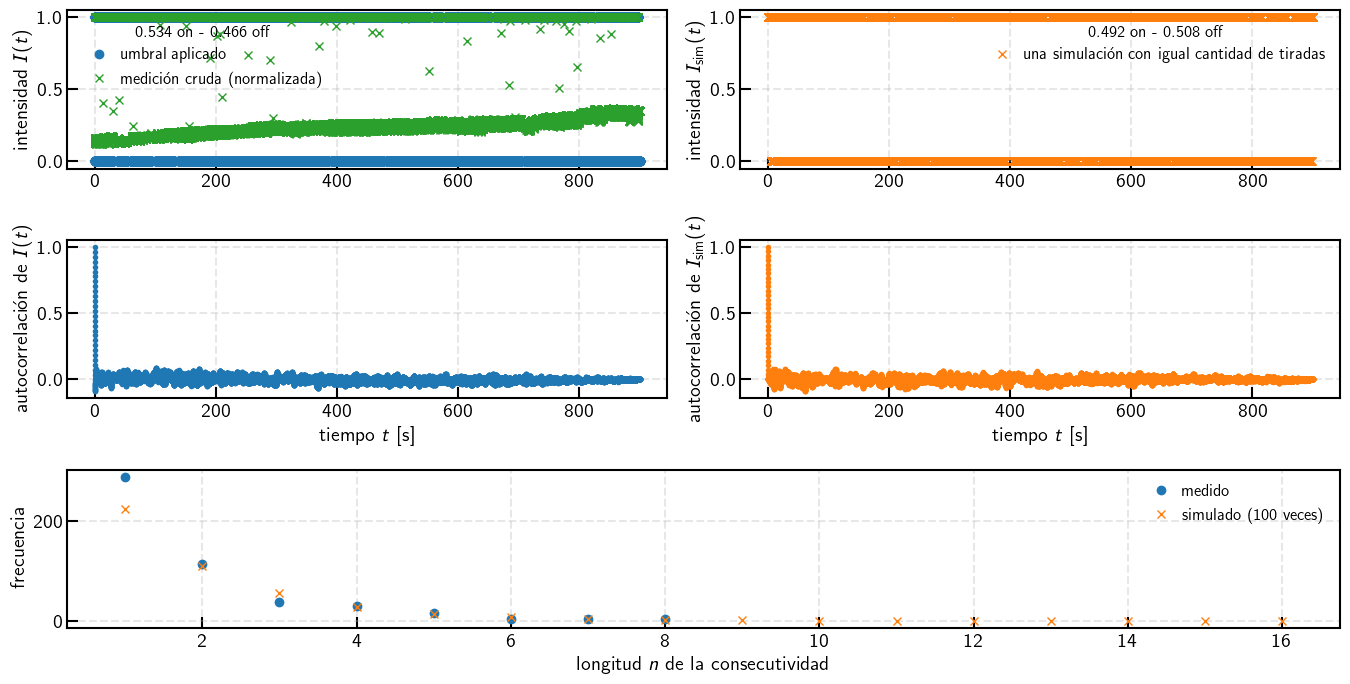
\includegraphics[width=\linewidth]{Resultados/15min_d.png}
	\caption{15 minutos, medición d.}
\end{figure}

\begin{figure}[!h]
	\centering
	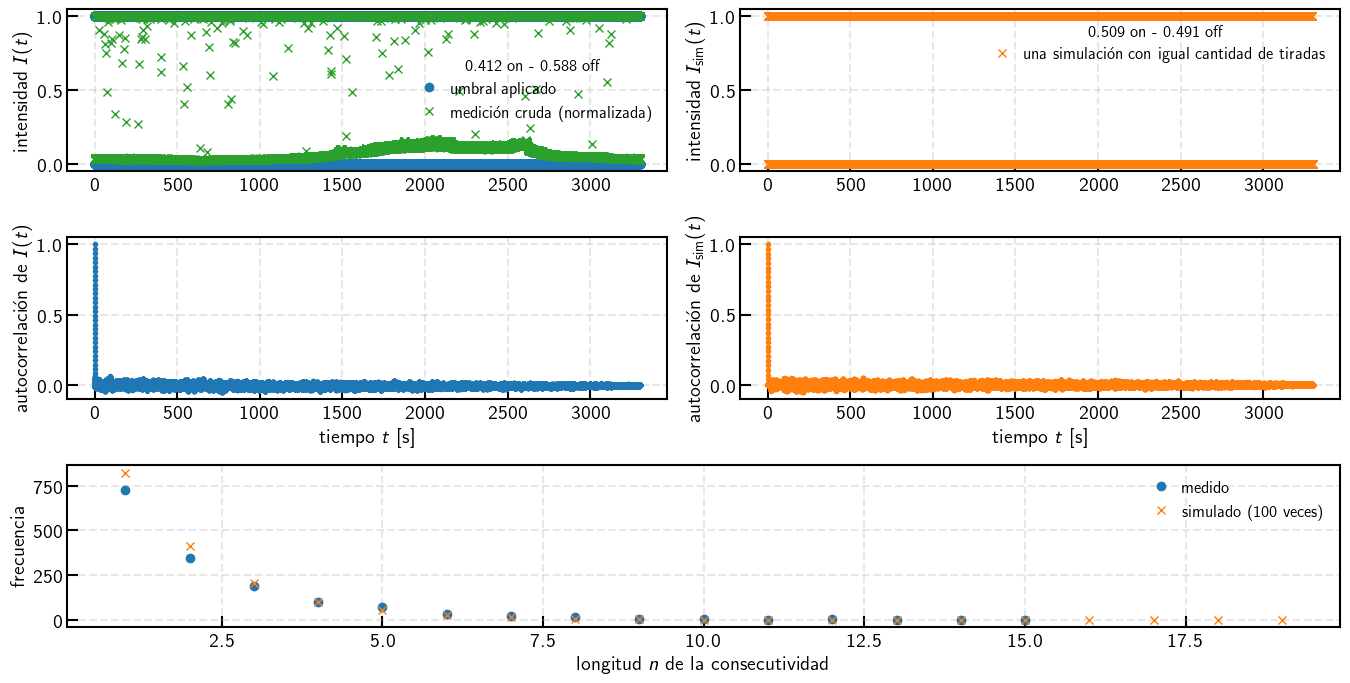
\includegraphics[width=\linewidth]{Resultados/1h.png}
	\caption{1 hora.}
	\label{fig:1hora}
\end{figure}

Me resisto a concluir que el generador de números aleatorio del Kilobot sea tan bueno como muestra la figura~\ref{fig:buena_moneda}.
Por ejemplo, en la figura~\ref{fig:1hora} donde grabamos una hora la proporción on/off es 40/60 cuando, a mayor cantidad de tiradas ($3600$ en este caso), debería ser casi 50/50.
Y aunque en otras mediciones, ya no hay TAN buena correspondencia en las frecuencias medidas y simuladas, para $n \leq 3$, \emph{sí} la hay para longitudes grandes, pero nosotros \textbf{vimos} al Kilobot girando $10$, $11$ o $12$ veces en un mismo sentido.
Ahora sospecho que ponerlo en movimiento pueda afectar su ``moneda''.
Por eso pasamos a caracterizar la ``moneda'' en movimiento: vamos a cargar un programa que active los motores \emph{y} prenda el LED.

Lo peor que pasó fue la proporción on/off que obtuvimos (cuando contábamos con 2 Kilobots) el primer día:

\begin{figure}[!h]
	\centering
	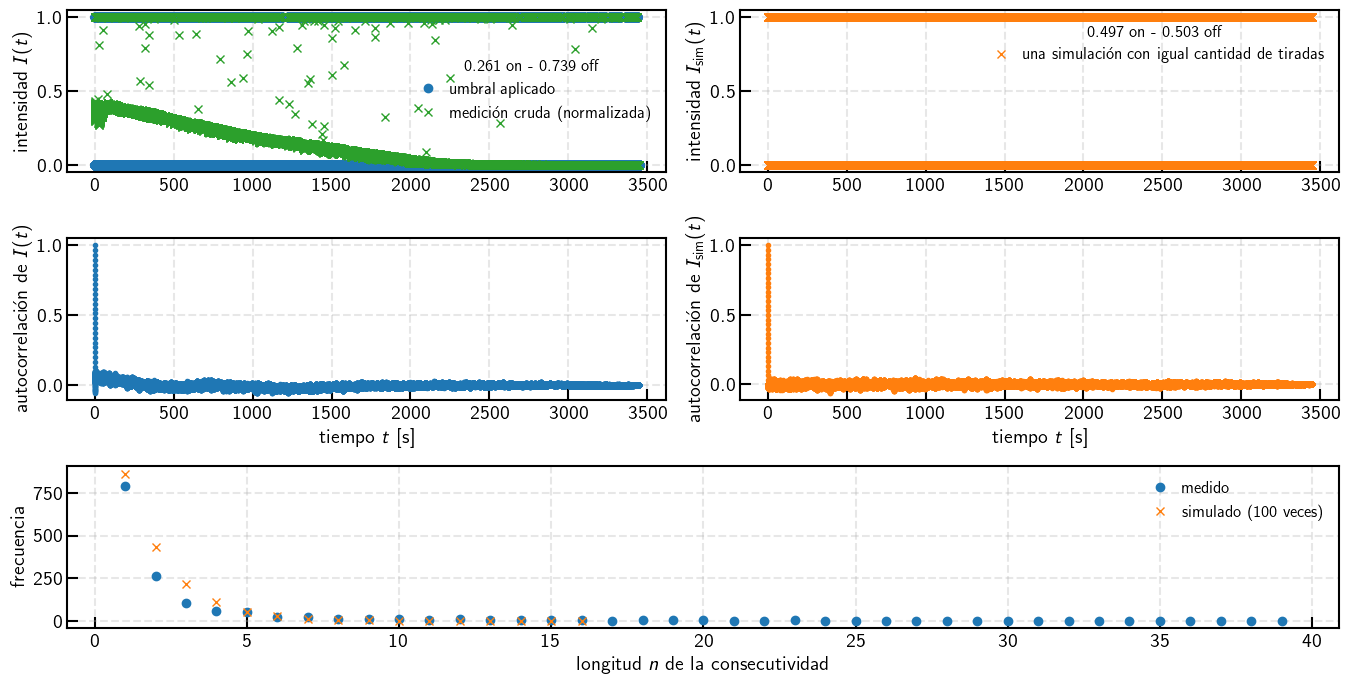
\includegraphics[width=\linewidth]{Resultados/1h_soft.png}
	\caption{1 hora con el Kilobot nuevo.}
	\label{fig:1hora_soft}
\end{figure}

\begin{figure}[!h]
	\centering
	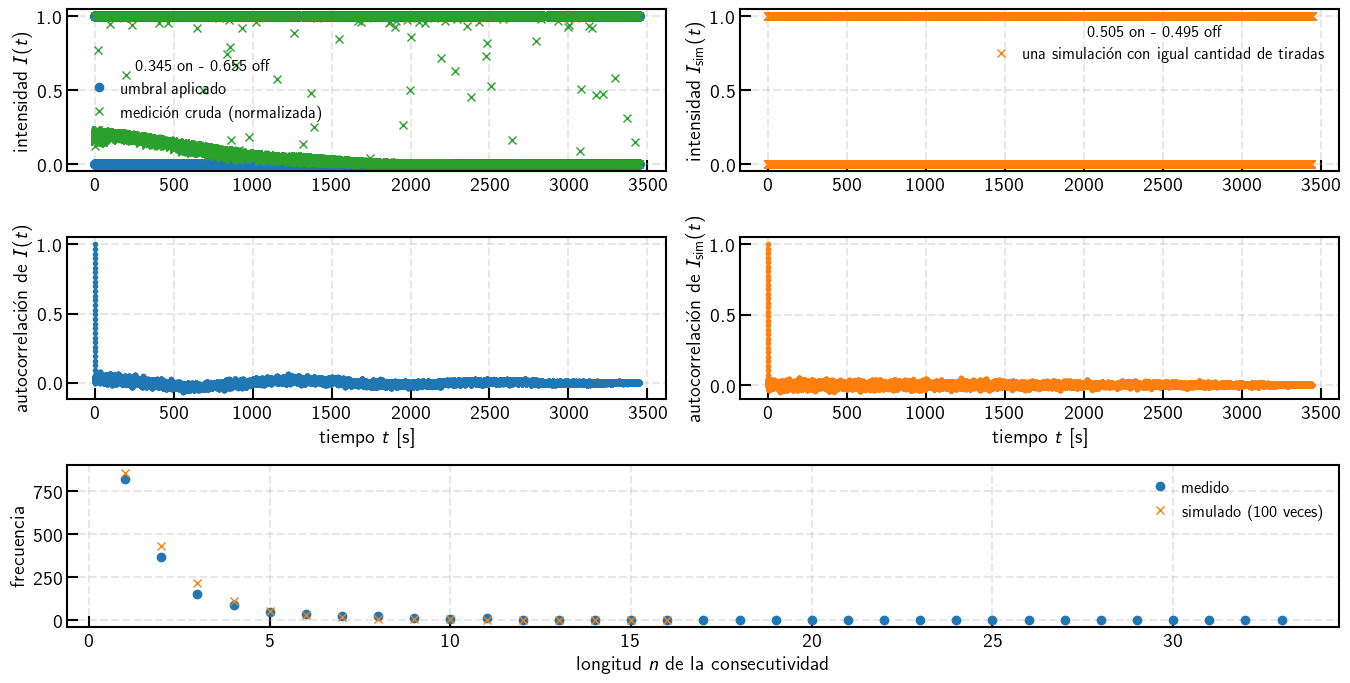
\includegraphics[width=\linewidth]{Resultados/1h_hard.png}
	\caption{1 hora con el Kilobot al que Germán le cambió la batería. Por eso usamos \texttt{rand\_soft()} (sin seed) aunque seguro no tenga nada que ver.}
	\label{fig:1hora_hard}
\end{figure}

Vemos la horrible proporción 30/70 y aun más sorprendente que se presentan consecutividades muuuy grades con $n>30$ (!!), mientras que en $100$ simulaciones la máxima fue de $n_\mathrm{max} = 16$.
Si vemos los gráficos anteriores, se presenta el caso contrario: mayores $n$ se presentan cuando simulamos ya que le damos 100 tiradas de changüí para que estas aparezcan.

Algo pasó ese día y no sabemos qué.
Desde la última de medición de Labo 7 no habíamos tocado a los Kilobots y para esa primera medición volvimos a prenderlos.
El programa que le cargamos y el controlador son lo único que tuvieron en común esos dos Kilobots que después titilaban independientemente.
A las semanas siguiente se rectificó.

Otra cosa que nos dimos cuenta al simular la moneda y contar las consecutividades, es que la frecuencia~$f$ en función de la longitud $n$ pareciera seguir una forma del tipo $f(n) \propto \frac{1}{2^n}$.
No sabemos si este problema está resuelto exactamente (\url{https://math.stackexchange.com/questions/977063/exactly-k-consecutive-heads-n-tosses}).
\href{https://math.stackexchange.com/questions/148353/given-n-raffles-what-is-the-chance-of-winning-k-in-a-row}{Acá} y \href{https://marknelson.us/posts/2011/01/17/20-heads-in-a-row-what-are-the-odds.html}{acá} llegan a una fórmula que involucra a la sucesión de Fibonacci pero ahí consideran que, por ejemplo, en HHHT se produce un consecutividad de $n=2$ porque dentro de las HHH salieron dos caras consecutivas.
Pero en nuestro caso la longitud de la consecutividad tiene que ser exacta, o sea, para nosotros $f(n=1)=1$, $f(n=2)=0$ y $f(n=3)=1$.
También el enunciado de su problema sólo considera las caras, pero nosotros contamos la contribución de caras \emph{y} cecas.
Aunque esto último se puede arreglar si modificamos nuestro simulador y lo ponemos a contar consecutividad de sólo caras.
O si hay alguna fórmula que dé la probabilidad de tener \emph{exactamente} $n$ caras consecutivas en $N$ tiradas, el problema con caras y cecas se resuelva con agregando un factor $2$ aunque esto lo veo muy optimista.

La fórmula a la que llegó en el último link es terrible y no sé si una fórmula que resuelva nuestro problema es fácil de obtener.
O tal vez sí y es un ejercicio de la guía de Proba de Teo 3.

\end{document}
